\documentclass{beamer}
%Information to be included in the title page:
\title{House Prices - Advanced Regression Techniques}
\author{Luca Corsetti}
\institute{University of Bologna}
\date{2025}

\usepackage{minted}

\begin{document}

\frame{\titlepage}

\begin{frame}
\frametitle{Project Objective \& Approach}
To \textbf{build a regression model} that predicts the \textbf{sale price of houses} in Ames, Iowa, using advanced regression techniques.
\
The workflow followed these steps:

\begin{enumerate}
    \item Exploratory Data Analysis (EDA)
    \item Data cleaning and preprocessing
    \item Modeling \& Evaluation
    \item Bonus - Trying to improve the Kaggle score
\end{enumerate}
\end{frame}

\begin{frame}
\frametitle{The Dataset}
\begin{itemize}
    \item \textbf{1460} training samples with \textbf{79} features describing various aspects of residential homes
    \item Mixed data types: \textbf{numerical} (e.g GrLivArea), \textbf{categorical} (e.g Neighborhood), \textbf{ordinal} (e.g OverallQual)
    \item Target variable in the train.csv dataset: **SalePrice**
\end{itemize}
\end{frame}

\begin{frame}
\frametitle{Dataset Exploration: the target variable \textbf{SalePrice}}
\centering
    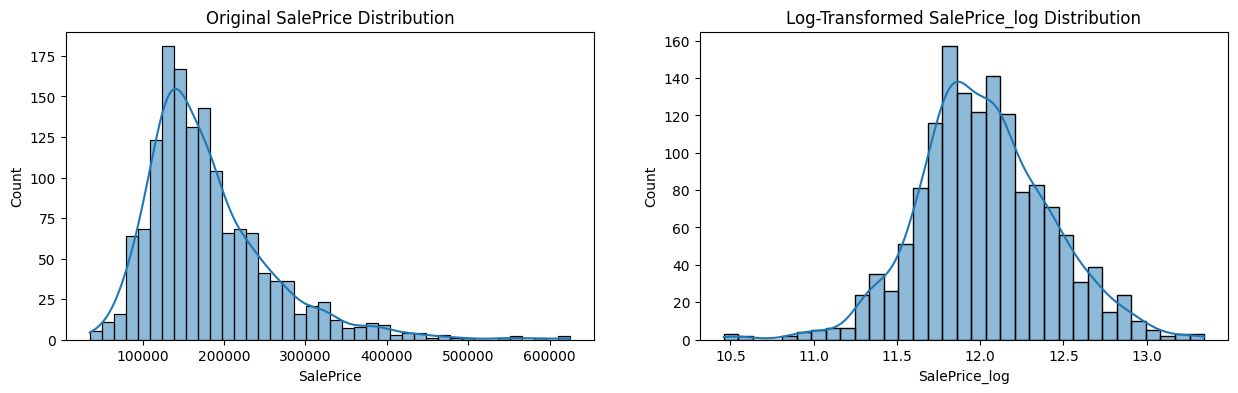
\includegraphics[width=1\textwidth]{../challenge/main_files/main_30_0.png}

\begin{itemize}
    \item Right-skewed distribution
    \item Solution: Apply log transformation to normalize the distribution
\end{itemize}
\end{frame}

\begin{frame}
\frametitle{Dataset Exploration: most influent features}
\centering
    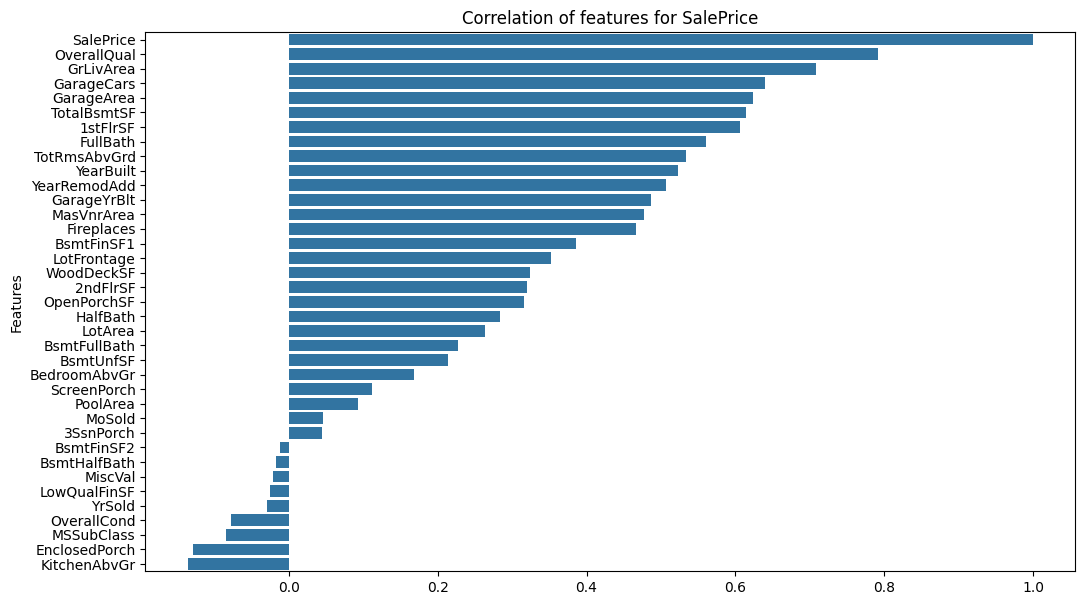
\includegraphics[width=.8\textwidth]{../challenge/main_files/main_17_0.png}

Most influential features based on correlation with SalePrice ($> 0.6$):
\begin{itemize}
    \item OverallQual ($0.79$) - ordinal
    \item GrLivArea ($0.71$) - numerical
    \item GarageCars ($0.64$) - numerical
    \item GarageArea ($0.62$) - numerical
    \item TotalBsmtSF ($0.61$) - numerical
\end{itemize}
\end{frame}

\begin{frame}
\frametitle{Dataset Exploration: outliers detection}
\centering
    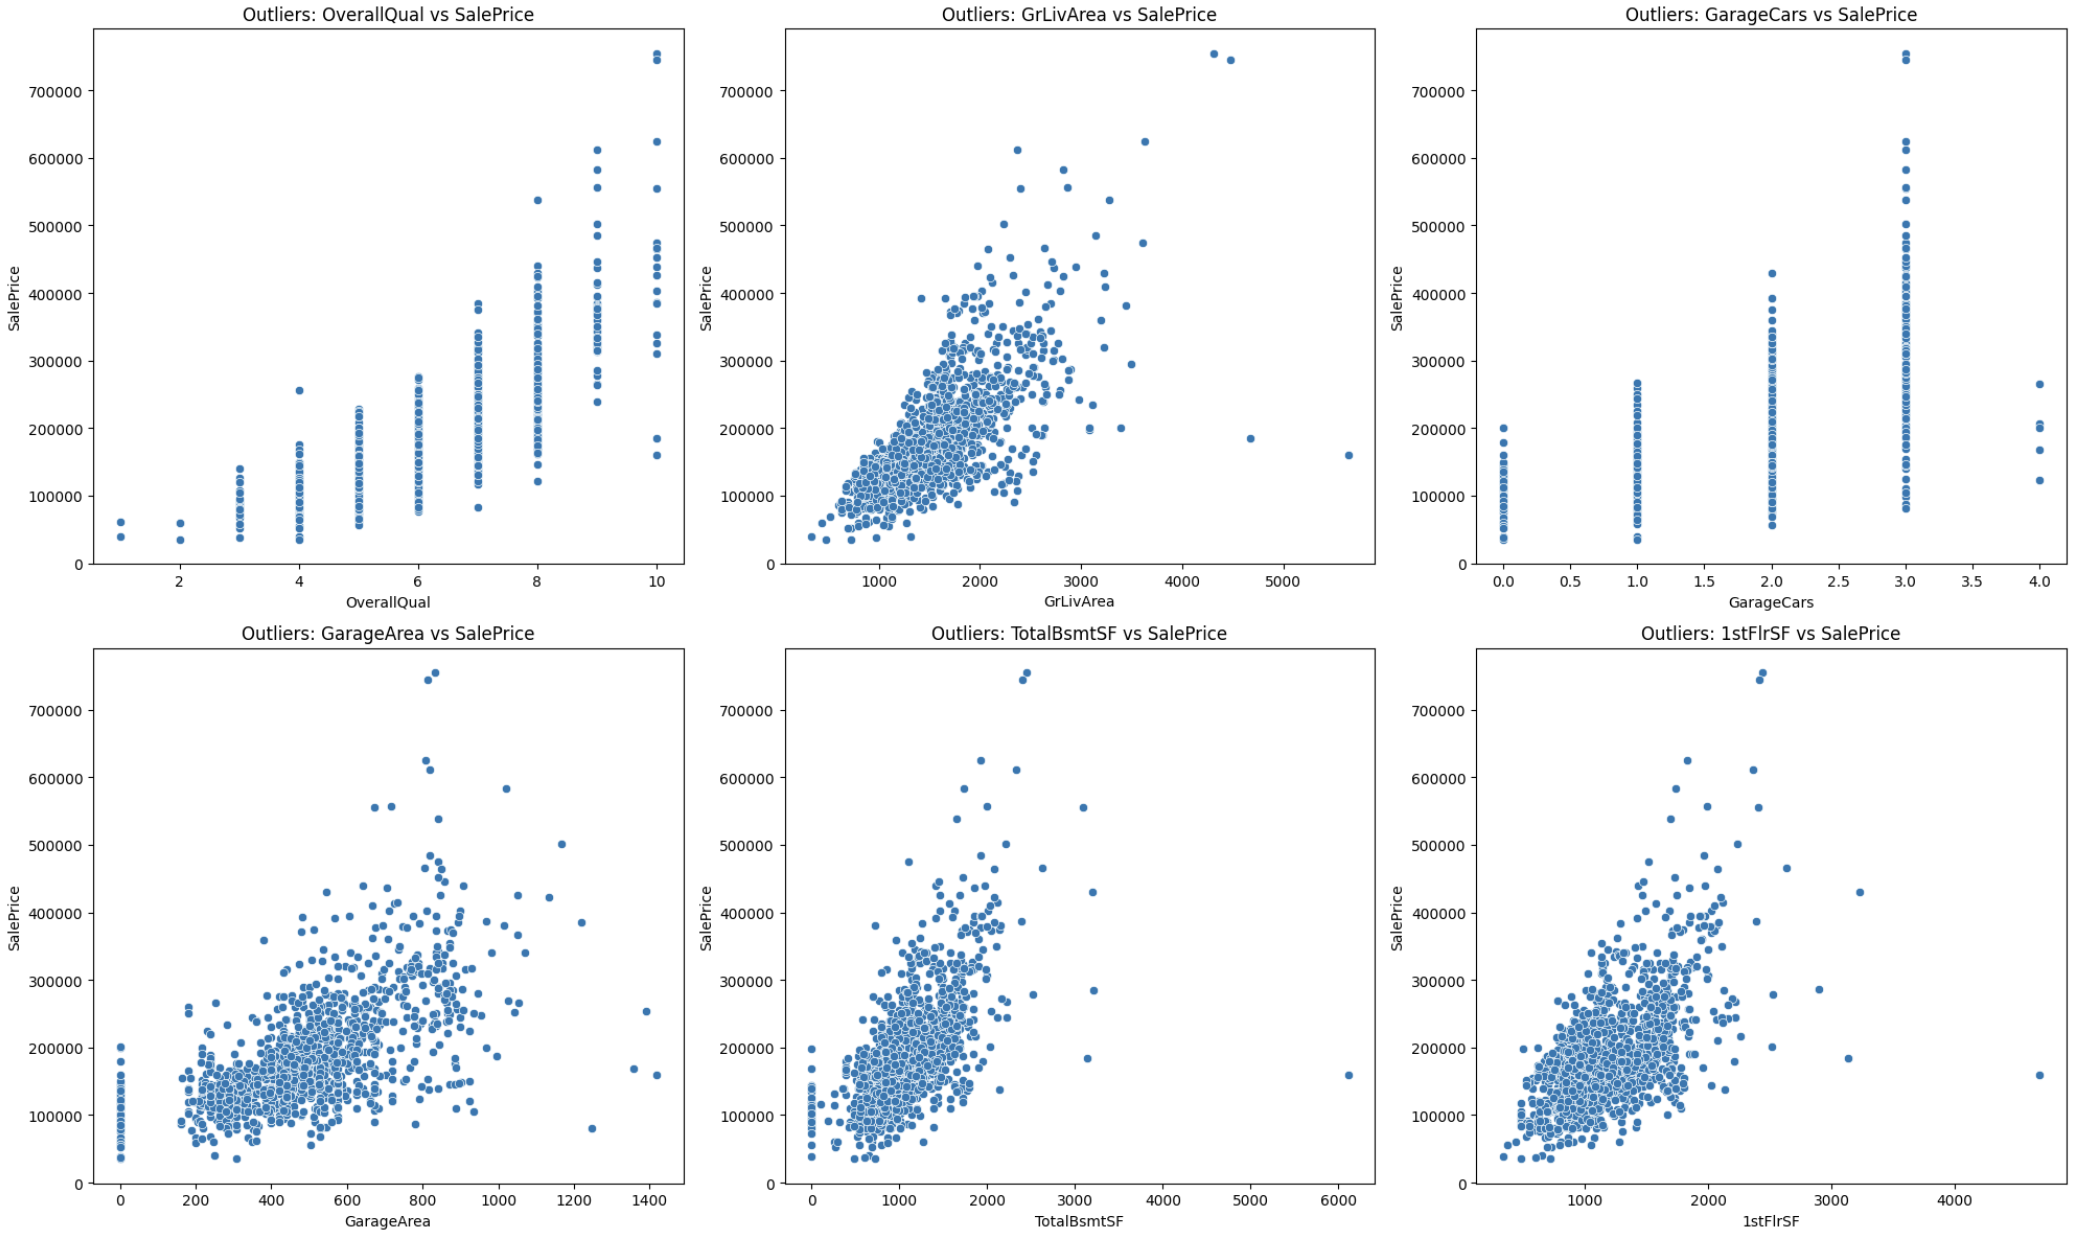
\includegraphics[width=.8\textwidth]{../challenge/main_files/main_92_0.png}

Solution: Remove outliers based on domain knowledge as they were likely data entry errors.
\end{frame}

\begin{frame}
\frametitle{Data Preparation: handling missing values}

\begin{itemize}
    \item Some features (e.g PoolQC, Alley, Fence) were read with \textbf{NaN} values because Pandas interpreted \textbf{None} as \textbf{NaN}. These features actually represent the absence of a feature, so they \textbf{should not be} removed.
    \item Whereas other features (e.g LotFrontage) have real missing values that need to be imputed. For this, the \textbf{median} of the feature was used.
\end{itemize}
\end{frame}

\begin{frame}
\frametitle{Data Preparation: feature encoding}

\begin{itemize}
    \item Ordinal features (e.g ExternalQual: Ex, Gd, TA, Fa and Po) need to be mapped to numerical values \textbf{based on their order}.
    \item Categorical features (e.g Neighborhood) are \textbf{one-hot encoded} to \textbf{create binary features} since there is no ordinal relationship between categories.
\end{itemize}

\end{frame}

\begin{frame}[fragile]
\begin{minted}[breaklines=true, fontsize=\tiny]{python}
# Ordinal encoding
from sklearn.preprocessing import OrdinalEncoder

qual_cols = ['ExterQual', 'ExterCond', 'BsmtQual', 'BsmtCond', 'HeatingQC', 'KitchenQual', 'FireplaceQu', 'GarageQual', 'GarageCond']
# other ordinal columns here ..

qual_encoder = OrdinalEncoder(categories=[qual_cats] * len(qual_cols), handle_unknown='use_encoded_value', unknown_value=-1)
# other ordinal encoders here ..

train_dataset_cleaned[qual_cols] = qual_encoder.fit_transform(train_dataset_cleaned[qual_cols])
# same with others
\end{minted}

\begin{minted}[breaklines=true, fontsize=\tiny]{python}
# Nominal encoding
from sklearn.preprocessing import OneHotEncoder

df_final['MSSubClass'] = df_final['MSSubClass'].astype(str)
df_test_final['MSSubClass'] = df_test_final['MSSubClass'].astype(str)

nominal_cols = df_final.select_dtypes(include=['object']).columns
ohe = OneHotEncoder(drop='first', sparse_output=False, handle_unknown='ignore')

# Fit on the training data and transform it
encoded_train = ohe.fit_transform(df_final[nominal_cols])
\end{minted}
\end{frame}

\begin{frame}
\frametitle{Modeling: strategy and metrics used}

\begin{itemize}
    \item Trained various regression models: Ridge, Random Forset, XGBoost
    \item Evaluated using Root Mean Squared Error (RMSE) and R-squared ($R^2$) metrics
    \item Fine-tuned hyperparameters using \textbf{GridSearchCV} with cross-validation (or \textbf{RandomSearchCV} to save time)
\end{itemize}
\end{frame}

\begin{frame}
\frametitle{Modeling: strategy and metrics used}

\footnotesize
$$\mathrm{error}=\mathrm{actual}-\mathrm{predicted}$$
$$\mathrm{MSE}=\frac{1}{n}\sum_{i=1}^{n}(\mathrm{actual}-\mathrm{predicted})^2$$
$$\mathrm{RMSE}=\sqrt{\mathrm{MSE}}=\sqrt{\frac{1}{n}\sum_{i=1}^{n}(\mathrm{actual}-\mathrm{predicted})^2}$$

$$\mathrm{SS}_{\mathrm{res}}(\mathrm{Sum\ of\ squared\ residuals})=\sum{i=1}^{n}(\mathrm{actual}-\mathrm{prediction})^2$$
$$\mathrm{SS}_{\mathrm{tot}}(\mathrm{Total\ sum\ of\ squares})=\sum{i=1}^{n}(\mathrm{actual}-\mathrm{mean})^2$$
$$R^2=1-\frac{\mathrm{SS}_{\mathrm{res}}}{\mathrm{SS}_{\mathrm{tot}}}$$
\normalsize
\end{frame}

\begin{frame}
\frametitle{Modeling: Ridge Regression}
\centering
    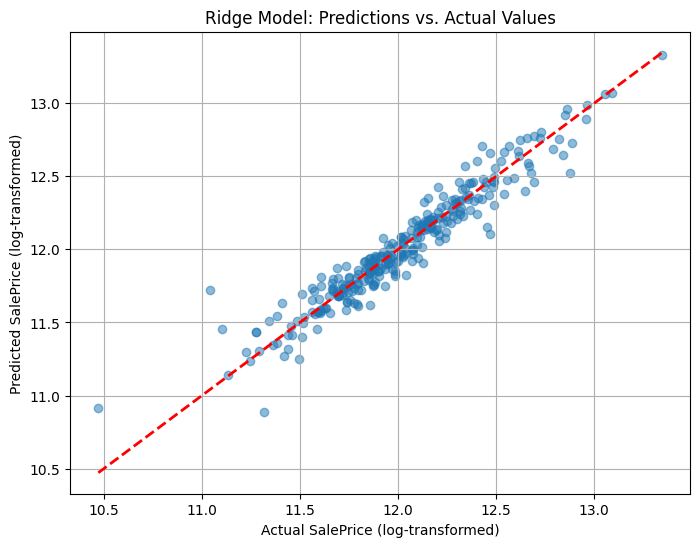
\includegraphics[width=.7\textwidth]{../challenge/main_files/main_45_0.png}

\begin{itemize}
    \item Why not \textbf{Linear Regression}? More robust to \textbf{multicollinearity} and \textbf{overfitting}
    \item Best hyperparameter $alpha=26.366508987303583$
    \item $RMSE = 0.1127$; $R^2 = 0.9192$ - not bad!
\end{itemize}
\end{frame}

\begin{frame}[fragile]
\frametitle{Modeling: Ridge Regression}

\begin{minted}[breaklines=true, fontsize=\tiny]{python}
from sklearn.model_selection import GridSearchCV

param_grid = {
    'alpha': np.logspace(-2, 3, 20) # generates a list of values from .01 to 1000
}

ridge_grid_search = GridSearchCV(
    estimator=Ridge(random_state=random_state),
    param_grid=param_grid,
    cv=5,
    scoring='neg_mean_squared_error' # take the negative of mse since GridSearchCV works by taking the best the highest value out of the estimation
)
\end{minted}
\end{frame}

\begin{frame}
\frametitle{Advanced Models: Random Forest \& XGBoost}
\centering
    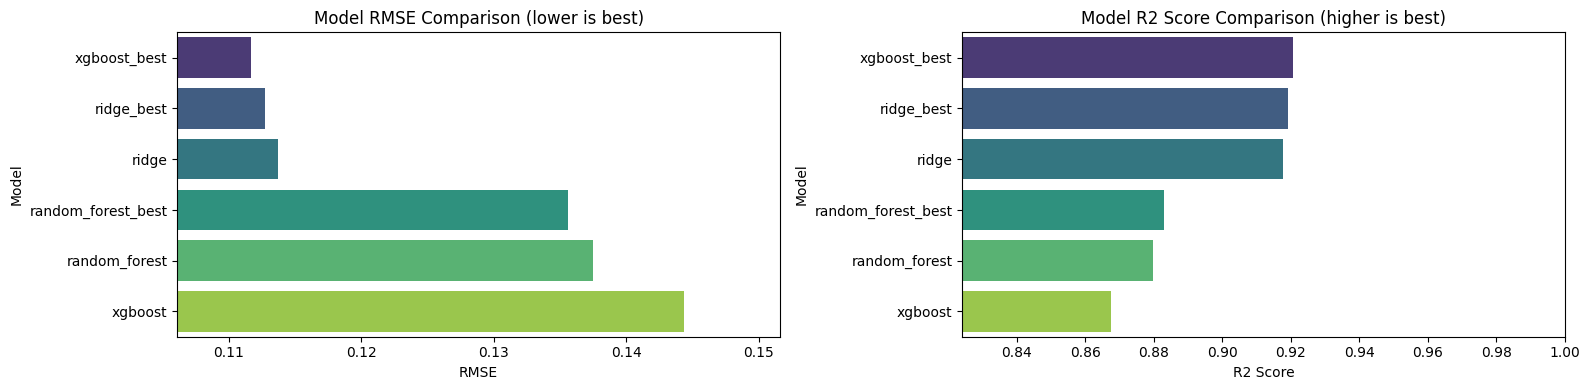
\includegraphics[width=1\textwidth]{../challenge/main_files/main_73_0.png}

\begin{itemize}
    \item \textbf{Tree based ensemble models} that can capture non-linear relationships and interactions between features
    \item Fine tuned hyperparameters of both, finding the \textbf{best model to be XGBoost}
\end{itemize}
\end{frame}

\begin{frame}[fragile]
\frametitle{Advanced Models: Random Forest \& XGBoost}

\begin{minted}[breaklines=true, fontsize=\tiny]{python}
from sklearn.model_selection import RandomizedSearchCV
import xgboost as xgb

param_grid = {
    'n_estimators': [100, 200, 300, 500],
    'max_depth': [10, 20, 30, None],
    'min_samples_split': [2, 5, 10],
    'min_samples_leaf': [1, 2, 4],
    'max_features': [1.0, 'sqrt']
}

rf_random_search = RandomizedSearchCV(
    estimator=RandomForestRegressor(random_state=random_state),
    param_distributions=param_grid,
    cv=5,
    scoring='neg_mean_squared_error',
    n_jobs=-1,
    random_state=random_state
)

# ..

param_grid = {
    'max_depth': [3, 4, 5],
    'learning_rate': [0.05, 0.1, 0.2],
    'n_estimators': [100, 200, 300],
    'subsample': [0.8, 1.0]
}

xgb_grid_search = GridSearchCV(
    estimator=xgb.XGBRegressor(random_state=random_state),
    param_grid=param_grid,
    cv=5,
    scoring='neg_mean_squared_error',
    n_jobs=-1
)
\end{minted}
\end{frame}

\begin{frame}
\frametitle{Submitting to Kaggle}

\begin{itemize}
    \item For this competition, Kaggle uses \textbf{RMSE} to evaluate the predictions on the test set
    \item Submitting the predictions of the XGBoost best model to Kaggle placed me in \textbf{$1172^{th}$} position with a score of \textbf{$0.12810$}
    \item \textbf{Can we do better?}
\end{itemize}
\end{frame}

\begin{frame}[fragile]
\frametitle{Submitting to Kaggle}

\begin{minted}[breaklines=true, fontsize=\tiny]{python}
def create_submission(model, X_train_full, y_train_full, X_test_full, output_file_name='submission'):
    params = model.get_params()
    model_type_name = type(model).__name__

    model = None

    match model_type_name:
        case 'Ridge':
            model = Ridge(**params)
        case 'RandomForestRegressor':
            model = RandomForestRegressor(**params)
        case 'XGBRegressor':
            model = xgb.XGBRegressor(**params)
        case _:
            print(f"Error: Unhandled model type '{model_type_name}'")
            return

    model.fit(X_train_full, y_train_full)
    print("Retraining complete.")
    
    X_test_prepared = X_test_full.copy()
    
    print("Making predictions on the prepared test set...")
    final_predictions_log = model.predict(X_test_prepared)
    
    final_predictions = np.expm1(final_predictions_log)
    
    submission = pd.DataFrame({'Id': X_test_prepared.index, 'SalePrice': final_predictions})
    submission.to_csv(f'{output_file_name}.csv', index=False)
\end{minted}
\end{frame}

\begin{frame}[fragile]
\frametitle{Improving: Feature Engineering}
\begin{itemize}
    \item Noticed that I could've created more meaningful features from the existing ones
    \item Created new features like TotalSF (Total Square Footage), TotalBathrooms, Age, etc. that aggregate existing features into one.
\end{itemize}

\begin{minted}[breaklines=true, fontsize=\tiny]{python}
def add_features(df):
    df['TotalSF'] = df['TotalBsmtSF'] + df['1stFlrSF'] + df['2ndFlrSF']
    df['TotalBath'] = df['FullBath'] + 0.5 * df['HalfBath'] + df['BsmtFullBath'] + 0.5 * df['BsmtHalfBath']
    df['TotalPorchSF'] = df['OpenPorchSF'] + df['EnclosedPorch'] + df['3SsnPorch'] + df['ScreenPorch']

    df['HouseAge'] = df['YrSold'] - df['YearBuilt']
    df['RemodelAge'] = df['YrSold'] - df['YearRemodAdd']

    df['IsNew'] = (df['YrSold'] == df['YearBuilt']).astype(int)
    df['WasRemodeled'] = (df['YearRemodAdd'] != df['YearBuilt']).astype(int)

    df['OverallQual_x_TotalSF'] = df['OverallQual'] * df['TotalSF']
    df['OverallQual_x_HouseAge'] = df['OverallQual'] * df['HouseAge']

    return df
\end{minted}
\end{frame}

\begin{frame}
\frametitle{Improving: Feature Engineering}
\centering
    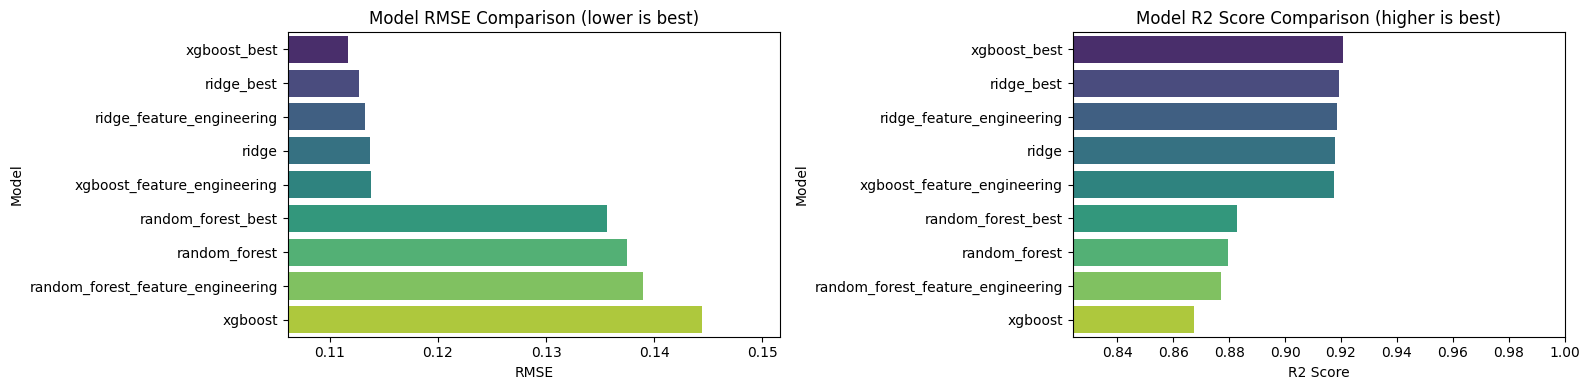
\includegraphics[width=.9\textwidth]{../challenge/main_files/main_85_0.png}

\begin{itemize}
    \item \textbf{Retrained the models with the new features}, surprisingly none of them improved the score.
\end{itemize}
\end{frame}

\begin{frame}
\frametitle{Improving: Stacking}

\begin{itemize}
    \item Stacking is an ensemble learning technique that \textbf{combines multiple models} to improve predictive performance \textbf{by training a meta-model on their outputs}.
    \item Used Ridge, Random Forest and XGBoost as base models and trained a \textbf{Ridge regression as meta-model}.
\end{itemize}
\end{frame}

\begin{frame}
\frametitle{Improving: Stacking}
\centering
    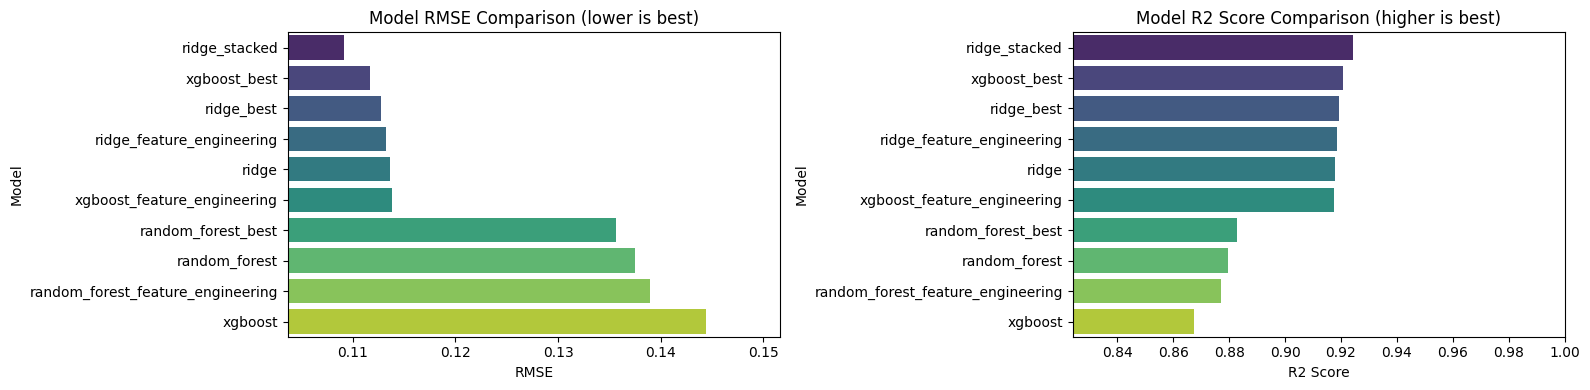
\includegraphics[width=.9\textwidth]{../challenge/main_files/main_91_1.png}

\begin{itemize}
    \item Retrained the models using Cross-Validation to generate out-of-fold predictions for the training set.
    \item Trained the meta-model on these predictions.
    \item Final Kaggle score after stacking: $0.12624$, which placed me in the $829^{th}$ position!
\end{itemize}
\end{frame}

\begin{frame}[fragile]
\frametitle{Improving: Stacking}

\begin{minted}[breaklines=true, fontsize=\tiny]{python}
base_models = [models['ridge_best']['model'], models['xgboost_best']['model'], models['random_forest_best']['model']]
base_model_names = ['ridge_best', 'xgboost_best', 'random_forest_best']

models['ridge_stacked'] = {
    'model': None,
    'prediction': None,
    'metrics': {}
}

models['ridge_stacked']['model'] = RidgeCV()

kf = KFold(n_splits=5, shuffle=True, random_state=random_state)

meta_features_train = np.zeros((X_train.shape[0], len(base_models)))
meta_features_test = np.zeros((X_test.shape[0], len(base_models)))

for i, model in enumerate(base_models):
    print(f"Processing base model {i+1}/{len(base_models)}: {base_model_names[i]}...")

    # Create out-of-fold predictions for training data
    for train_idx, val_idx in kf.split(X_train):
        model.fit(X_train.values[train_idx], y_train.values[train_idx])
        meta_features_train[val_idx, i] = model.predict(X_train.values[val_idx])

    # Create predictions for test data (by fitting on full training data)
    model.fit(X_train, y_train)
    meta_features_test[:, i] = model.predict(X_test)

models['ridge_stacked']['model'].fit(meta_features_train, y_train)
\end{minted}
\end{frame}

\begin{frame}
\frametitle{Conclusion}

\begin{itemize}
    \item \textbf{Dove deep} into data exploration and preprocessing to prepare the dataset for modeling.
    \item \textbf{Learned} about \textbf{XGBoost} and \textbf{ensemble methods} like stacking to improve model performance.
    \item Achieved a \textbf{final RMSE of $0.12624$} on Kaggle, placing me in the \textbf{$829^{th}$ position} out of \textbf{4925}.
\end{itemize}
\end{frame}

\end{document}
